\newpage
\subsection{Actividad 17}
Repetir el diseño en formato digital asumiendo un $T=0.05$,
partiendo de la función de transferencia discretizada del sistema y
polos deseados obtenidos a partir de la relación $z=e^{sT}$.

\lstinputlisting[language=MATLAB]{./codes/actividad17.m}

\begin{tcolorbox}[sharp corners, colframe=bluebox, title= Respuesta
  del sistema en tiempo discreto]
 % $>>>$ ltiview(\textcolor{blue}{`lsim'},kr*feedback(PDI\_10*Gposicionz,kr))
  \vspace*{0.35em}
  \mkanscode{
\begin{figure}[H]
  \centering
  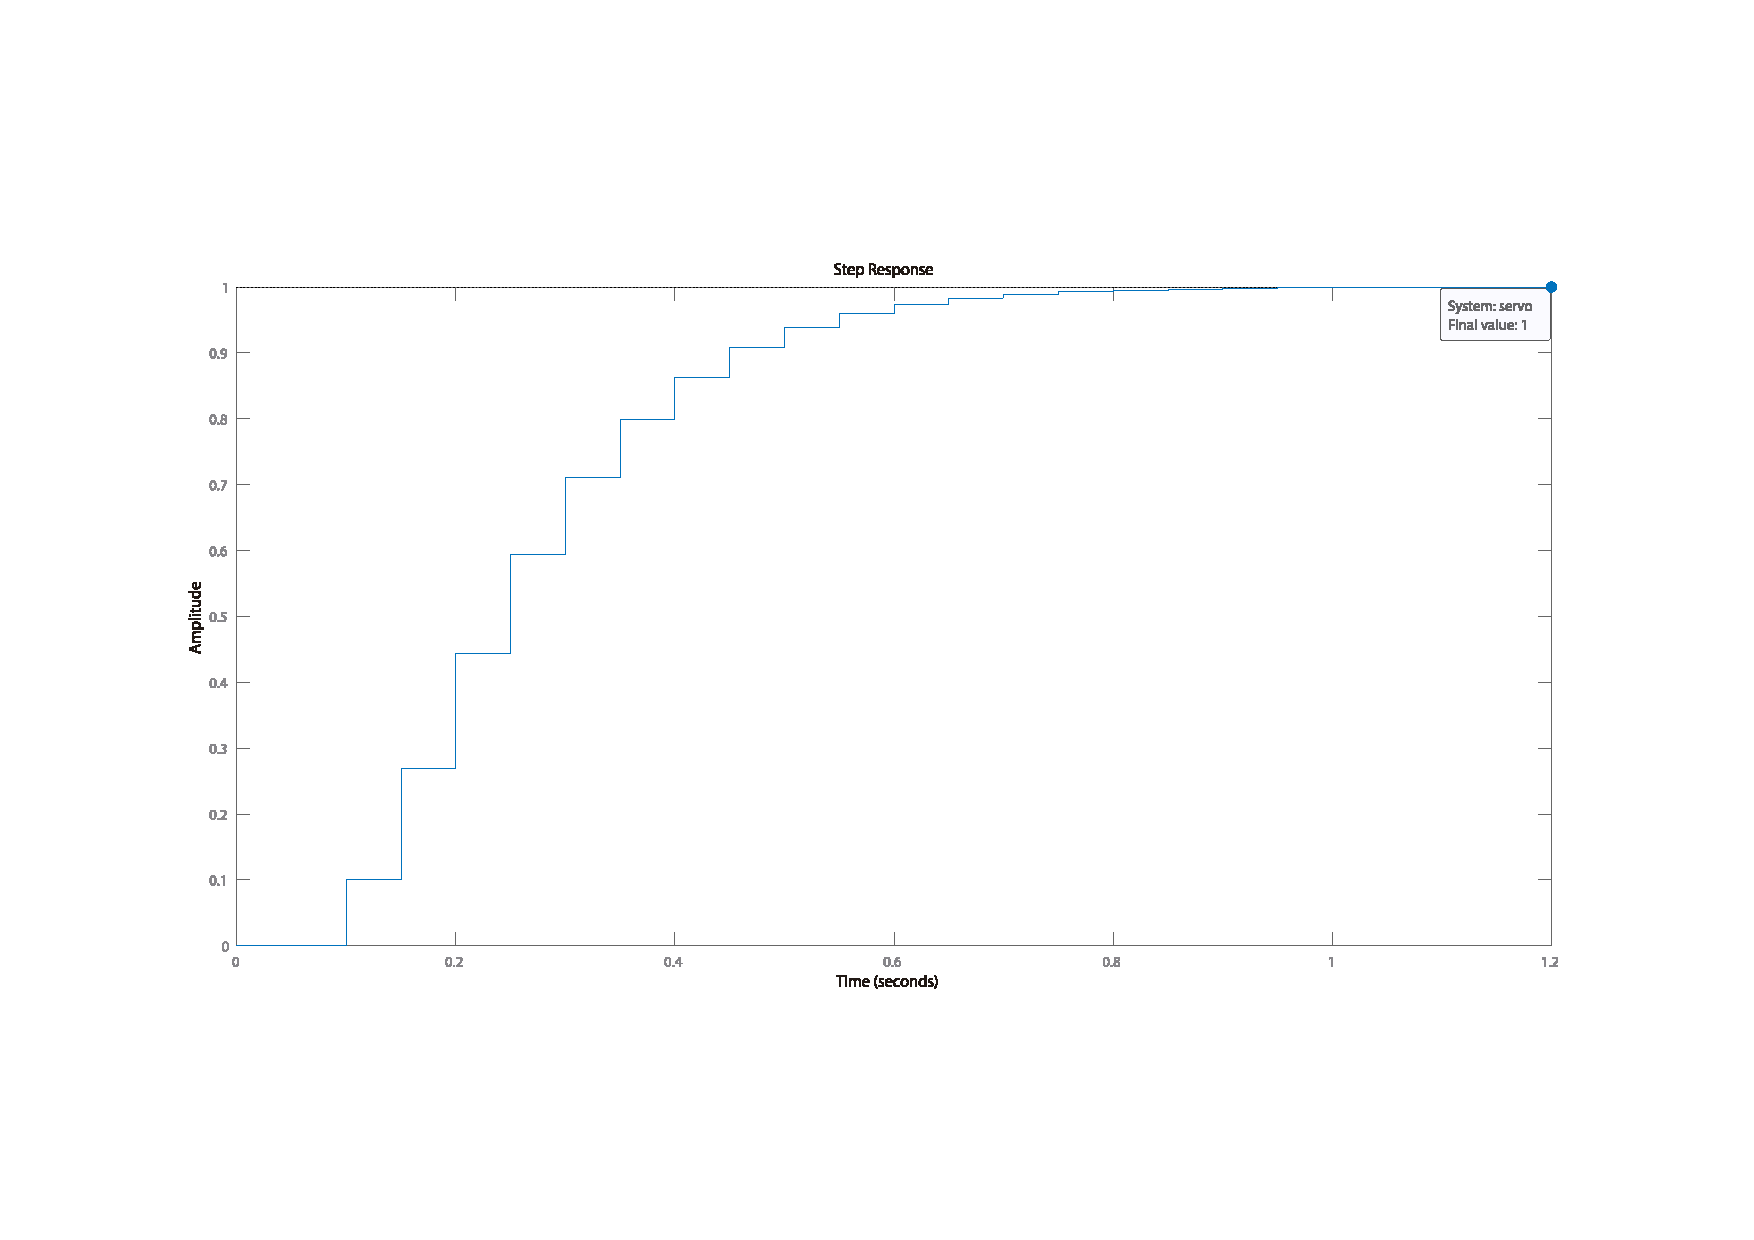
\includegraphics[clip, trim=2.5cm 4.5cm 2.5cm 4.25cm,
  scale=0.5]{images/figura 19.pdf}
  % izquierda,abajo,derecha,arriba
  \caption{Respuesta del sistema con error nulo.}
    \label{fig:figura 18}
\end{figure}
}
\vspace*{0.35em}
  \end{tcolorbox}%